\chapter{面向自动规划教学的积木世界VQA演示原型系统}
本章旨在设计并实现一个面向自动规划教学的积木世界VQA演示原型系统。
该系统基于本文提出的ABWG方法和RCNSP框架进行实现,
支持根据用户输入的以自然语言描述的部分可见积木世界生成指令和其它相关选项,临机生成部分可见积木世界图像或不同复杂度的部分可见积木世界演示数据集,
并能够完成积木世界的空间推理问答并展示思考过程,为开展自动规划课程的现场教学提供帮助。
下面分别从需求分析、架构设计、功能展示和集成测试四个方面进行详细阐述。
\section{需求分析}
本系统旨在基于本文提出的ABWG方法和神经符号VQA框架RCNSP,构建一个用于自动规划课堂教学演示的积木世界VQA原型系统。
该系统的基本任务包括以下几个方面:
\begin{enumerate}[nosep]
\item 根据用户输入的以自然语言描述的部分可见积木世界生成指令以及其它有关积木世界的选项,实现课堂场景下在较短时间内生成
部分可见积木世界图像或者不同复杂度的部分可见积木世界演示数据集。上述与有关积木世界的选项指的是一系列用户可以自定义的参数,
包括图像中物体数量、遮挡关系数量等等。
\item 在用户输入自然语言问题和积木世界的图像后,系统能够基于已有知识和图像中的信息,给出合理的回答。
并且能够在空间推理完成之后,展示推理的中间步骤和逻辑链条。
\item 为用户提供友好、直观的前端交互界面,便于课堂教学使用。
\end{enumerate}
\subsection{功能需求}
核心功能上,需要实现以下几个功能:
\begin{enumerate}[nosep]
\item 用户输入与对话处理。系统需要能够支持文本输入、图像输入,未来远期可以考虑加入语音输入。
此外,提供自动补全、拼写检查等输入辅助功能,以改善用户的输入体验。
\item 实时对话回复。系统能够通过DSPy的SDK,发起对本地LLM的调用,而LLM能够实时处理用户的问题,返回高质量的回答。
同时还应支持多轮对话,保持上下文关联,并具备记忆功能。
\item 对话历史记录。系统需要能够自动保存用户每次的对话记录,以供用户查看。
\item 帐户与认证。系统需要支持用户注册、登录、账号设置等功能。
\item 自定义生成不同复杂度的部分可见积木世界演示数据集。系统需要能够在控制台中允许用户可以自行调整生成积木世界VQA演示数据集的关键参数,以生成不同复杂度的演示数据。
\item 临机生成部分可见积木世界图像。当用户输入以自然语言描述的部分可见积木世界生成指令,同时选中一些有关积木世界的选项
(例如积木颜色取值范围、物体数量等)之后,系统能够在秒级时间内生成部分可见积木世界图像。
\end{enumerate}

辅助功能方面,主要围绕以下几点:
\begin{enumerate}[nosep]
\item 响应式设计。前端能够自适应桌面、平板和手机等不同设备。
\item 辅助说明。提供FAQ、帮助文档和使用指南,方便用户进行查阅。
\item 安全与异常处理。能够对恶意输入、不符合规范的输入进行拦截和提示。
\end{enumerate}
\subsection{非功能需求}
非功能需求主要聚焦于以下几个方面:
\begin{enumerate}[nosep]
\item 性能需求。系统需要能够在较短时间内完成对用户问题的回答,如果确实因为某些原因导致无法及时回答,需要能够给出合理的提示,
例如“正在思考...”等。另外,各个微服务应支持高并发访问,保证系统能够承受一定规模的大流量访问。
\item 可拓展性。对系统要按照主要功能来进行拆分,形成若干个微服务,
并且各个微服务之间要能够相互独立,实现松耦合。当系统需要进行拓展时,只需要增加新的微服务,而不需要对原有的微服务进行修改。
\item 可维护性。代码和文档需要保持清晰,易于理解和修改,特别是对于接口文档,要使用Swagger等工具进行规范化管理,以便于后续的维护和拓展。另外,要提供清晰的日志记录、监控报警机制,使用一些监控
工具,如Prometheus、Grafana等,对系统的运行状态进行监控,及时发现问题并解决。
\item 安全性。需对用户的数据传输与存储进行加密,尤其是手机号、密码等隐私信息应做脱敏处理,
以保证用户的隐私安全。此外,对登录、注册等操作,需要进行身份验证和权限控制,防止恶意攻击。此外,对于生成数据集的前端控制台,应该对参数的合法性进行前置校验,以免
攻击者利用非法参数向后台发起恶意攻击。
\item 可用性和用户体验。在整体外观上,系统需要提供简洁友好的用户图形界面,降低使用门槛。
\end{enumerate}

\section{架构设计}
\subsection{总体架构}
对本系统的总体架构设计如图\ref{fig:overall_architecture}所示。

后端部分采用微服务架构设计,包括视觉场景理解服务、语义解析服务、符号推理服务、规则修正服务、答案生成服务、
用户交互服务、日志与监控服务、数据存储服务等。各微服务之间通过API网关进行通信,API网关负责请求的路由、负载均衡、安全认证、限流等功能。

具体到各个微服务的主要职能如下:
\begin{enumerate}[nosep]
\item 视觉场景理解服务负责对用户上传的图片进行目标检测,并使用预定义谓词以 ASP 程序形式表示场景中的物体的相关信息。
\item 语义解析服务负责将用户的自然语言问题转化为ASP规则,以便于后续的推理。
\item 符号推理服务负责对ASP规则进行推理,得到问题的答案。
\item 规则修正服务负责对ASP规则进行修正。
\item 答案生成服务负责将符号推理服务输出的以ASP谓词表示的答案转化成自然语言。
\item 用户交互服务负责提供用户接口,接收用户的输入,调用其他服务,返回结果。
\item 日志与监控服务负责记录系统的运行日志,监控系统的运行状态,及时发现问题并解决。
\item 数据存储服务负责存储系统的数据,包括用户的信息、对话记录、ASP规则等。
\item 数据集生成服务负责根据数据生成前端控制台中传来的参数来生成数据集,同时也负责临机生成可控部分可见积木世界图像。
\end{enumerate}

前端部分,对UI界面的开发,选择Element UI框架,其具有丰富多样的按钮、输入框等搭建网页所需的元素,开发快捷方便。同时,使用Axios
向后端发送请求,实现前后端的数据交互。使用Vue构建组件化的前端页面,方便代码的维护和拓展。Vue Router用于实现前端路由,实现页面的跳转。Vuex用于实现状态管理,方便组件之间的数据传递。

在中间件上,系统引入了Sentinel进行流量控制,对系统的流量进行监控,实现限流、熔断等功能。RocketMQ用于实现消息队列,实现微服务之间的异步通信。
Redisson用于实现分布式锁,保证系统的并发安全。
\begin{figure}[h]
    \centering
    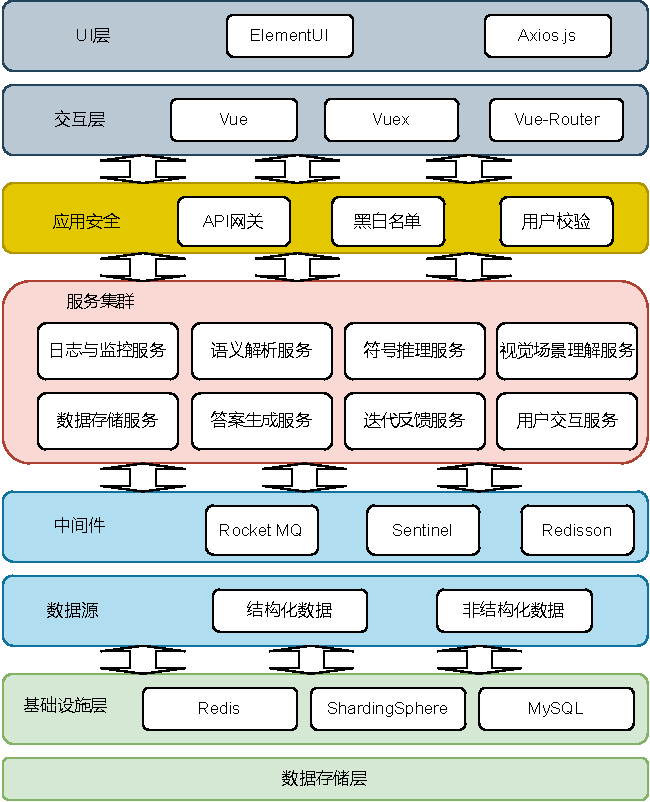
\includegraphics[scale=0.9]{figures/system_architecture-crop.pdf}
    \caption{系统总体架构}
    \label{fig:overall_architecture}
\end{figure}
\subsection{安全设计}
安全设计主要聚焦数据存储加密和传输安全,以确保系统的安全性和数据的机密性,防止数据泄露和未授权访问。

在存储加密上,针对数据库中存储了用户密码以及身份证号、手机号等高度敏感信息,根据字段的分类,采取不同措施,予以保护。
对于用户密码,采用SHA-256算法对明文密码进行加密后存储。对于除密码外的其它高度敏感字段(如身份证号、银行卡号),
使用AES加密函数,搭配密钥管理。

在传输安全上,采用HTTPS加密传输的方式,以防止中间人攻击。同时,使用JWT进行身份验证。
为了防止数据在传输过程中被篡改,使用HMAC-SHA256进行数据完整性校验。

\subsection{数据库设计}
设置User、Rule、Log、Dialog以上四个数据库。下面,对这四个数据库的职责及内设表进行介绍。

User数据库主要用于存储用户、角色、权限、会话信息等。内部包含如下表:
\begin{enumerate}[nosep]
\item 用户表users,用于存储用户信息。
\item 用户组表roles,用于存储用户组信息。
\item 用户组关系表user\_roles用于存储用户与用户组之间关系。
\item 用户状态表user\_session,用于存储会话或者登录状态记录。
\end{enumerate}
Rule数据库专门用于存储ASP规则及其相关信息。内部包含rules表和rule\_conditions表。rules表为主规则表,rule\_conditions表为规则条件表。具体表字段见
表\ref{tab:rule}。
\begin{table}[h]
    \centering
    \renewcommand{\arraystretch}{1.3} % 调整行间距
    \resizebox{\textwidth}{!}{
    \begin{tabular}{|l|l|l|}
        \hline
        \textbf{字段名称} & \textbf{数据类型} & \textbf{说明} \\ 
        \hline
        rule\_id & INT AUTO\_INCREMENT PRIMARY KEY & 规则唯一标识 \\ 
        \hline
        rule\_name & VARCHAR(255) & 规则名称 \\ 
        \hline
        rule\_head & VARCHAR(255) & 规则若论部分 \\ 
        \hline
        priority & INT & 优先级 \\ 
        \hline
        status & ENUM('active', 'inactive') & 状态标识 \\ 
        \hline
        description & TEXT & 描述或备注 \\ 
        \hline
        created\_at & DATETIME DEFAULT CURRENT\_TIMESTAMP & 创建时间 \\ 
        \hline
        updated\_at & DATETIME DEFAULT CURRENT\_TIMESTAMP ON UPDATE CURRENT\_TIMESTAMP & 更新时间 \\ 
        \hline
    \end{tabular}
    }
    \caption{rule表字段设置及说明}
    \label{tab:rule}
\end{table}
\begin{table}[h]
    \centering
    \renewcommand{\arraystretch}{1.3} % 调整行间距
    \resizebox{\textwidth}{!}{
    \begin{tabular}{|l|l|l|}
        \hline
        \textbf{字段名称} & \textbf{数据类型} & \textbf{说明} \\ 
        \hline
        condition\_id & INT AUTO\_INCREMENT PRIMARY KEY & 条件唯一标识 \\ 
        \hline
        rule\_id & INT & 外键,关联到主规则表 \\ 
        \hline
        condition\_text & VARCHAR(255) & 单个条件表达式,例如"X > 10" \\ 
        \hline
        sequence & INT & 条件顺序号,用于保持条件排列 \\ 
        \hline
        created\_at & DATETIME DEFAULT CURRENT\_TIMESTAMP & 创建时间 \\ 
        \hline
        updated\_at & DATETIME DEFAULT CURRENT\_TIMESTAMP ON UPDATE CURRENT\_TIMESTAMP & 更新时间 \\ 
        \hline
    \end{tabular}
    }
    \caption{rule\_condition表字段设置及说明}
    \label{tab:rule_conditions}
\end{table}

Log数据库存储系统运行日志、错误日志、操作记录等信息。其内部包含如下表:
\begin{enumerate}[nosep]
\item 系统日志表system\_logs,用于记录系统一般日志。
\item 错误日志表error\_logs,用于记录错误信息。
\item 审计日志表audit\_logs,用于记录关键操作审计日志。
\end{enumerate}

Dialog数据库存储所有用户与系统的对话记录。其内部包含如下表:
\begin{enumerate}[nosep]
\item 对话主表dialogs,用于记录每个对话的基本信息。
\item 对话消息表dialog\_messages,用于存储对话中用户发出的消息与LLM给出的每条回复。
\end{enumerate}

\subsection{缓存设计}
为系统使用缓存的目标包含以下两点:
\begin{enumerate}[nosep]
\item 提高响应速度。在整个VQA系统中,需要LLM参与的语义解析、
规则修正以及视觉场景理解环节,所需时间较长,目前较难以大幅度优化。为尽可能减少模型调用次数、提高响应速度并改善用户体验,系统引入了缓存机制;
\item 降低后端负载。如果访问量超出系统的承载能力,可能会导致部分服务宕机。以 Redis 为代表的缓存,其单机 QPS 可达 10 万,远超数据库等请求链路上的其它环节的承载能力。引入缓存,可一定程度上减少
对数据库和LLM的直接访问次数,缓解VQA系统在高并发场景下的压力。
\end{enumerate}

为了更好地做到成本与性能之间的平衡,本文采用了多层次缓存架构,共分两层。

第一层是本地内存缓存,用于缓存短生命周期、访问频率非常高的数据,如最近对话状态、会话上下文的部分数据。
在实现方式上,使用Java的ConcurrentHashMap配合LRU算法对缓存进行管理。

第二层是分布式缓存,本系统选用Redis,用于缓存跨多个服务器共享的数据,如会话历史、用户信息、通用问答的缓存结果等。
分布式缓存可以保证在集群环境下数据的一致性和高可用性,并支持数据持久化和数据过期策略。至于选用
Redis作为分布式缓存的理由,是因为其支持丰富的数据结构、持久化存储和分布式部署,同时具有高性能。

\section{功能展示}
\subsection{积木世界VQA问答}
积木世界VQA问答的前端主页面如图\ref{fig:welcome-page}所示,采用了模仿ChatGPT的网页样式。
用户可在界面中自行选择模型,包括本文的RCNSP框架中的微调后的模型、OpenAI的GPT系列模型、Google的Gemini系列模型、Meta的LLaMA系列模型
以及阿里巴巴的QWen系列模型,默认选用本文的微调后模型。
用户可以在下方的菜单栏中,点击第二个按钮,以上传图片。同时,历史对话也会在左侧栏中予以显示。
输入框旁配有语音输入按钮,点击后将调用百度语音识别 API,为用户提供语音输入服务。
上传图片并提出问题、系统给予答复后的效果如图\ref{fig:question}所示。
用户发送的文本和图片将会在同一个消息框内显示。用户要求系统重新生成回复,或者引用系统的某条回复,以让系统能够更加贴合用户的语境。

用户所提出的问题的思考过程和逻辑链条,默认情况下不展示。如果要查看,用户可通过双击模型给出的回复,
系统将会在同一个回复框中,展示推理过程中所用的视觉场景理解所得ASP规则、所用的谓词、问题语义解析所得ASP规则以及推理的链式流程,如图\ref{fig:answer}所示。
\begin{figure}[h]
    \centering
    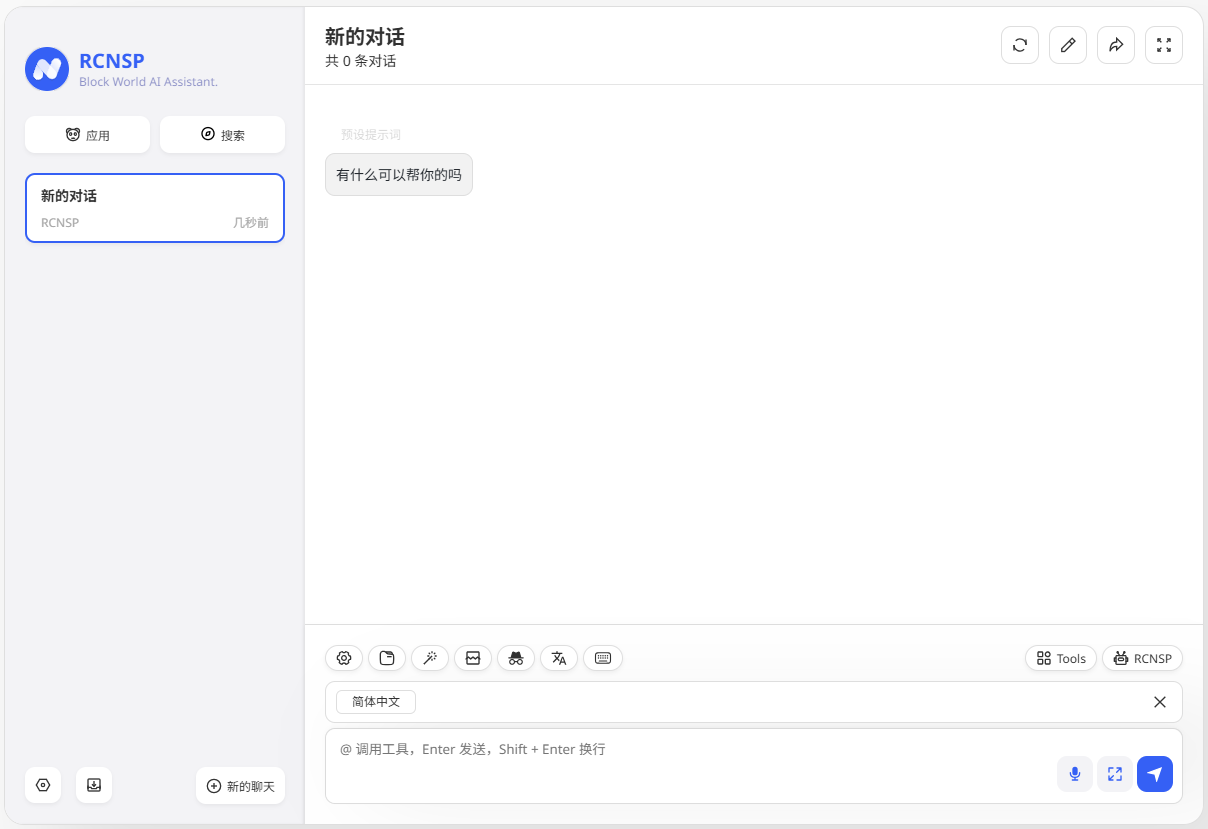
\includegraphics[scale=0.35]{figures/frontend-welcome-page.png}
    \caption{新对话页面}
    \label{fig:welcome-page}
\end{figure}
\begin{figure}[h]
    \centering
    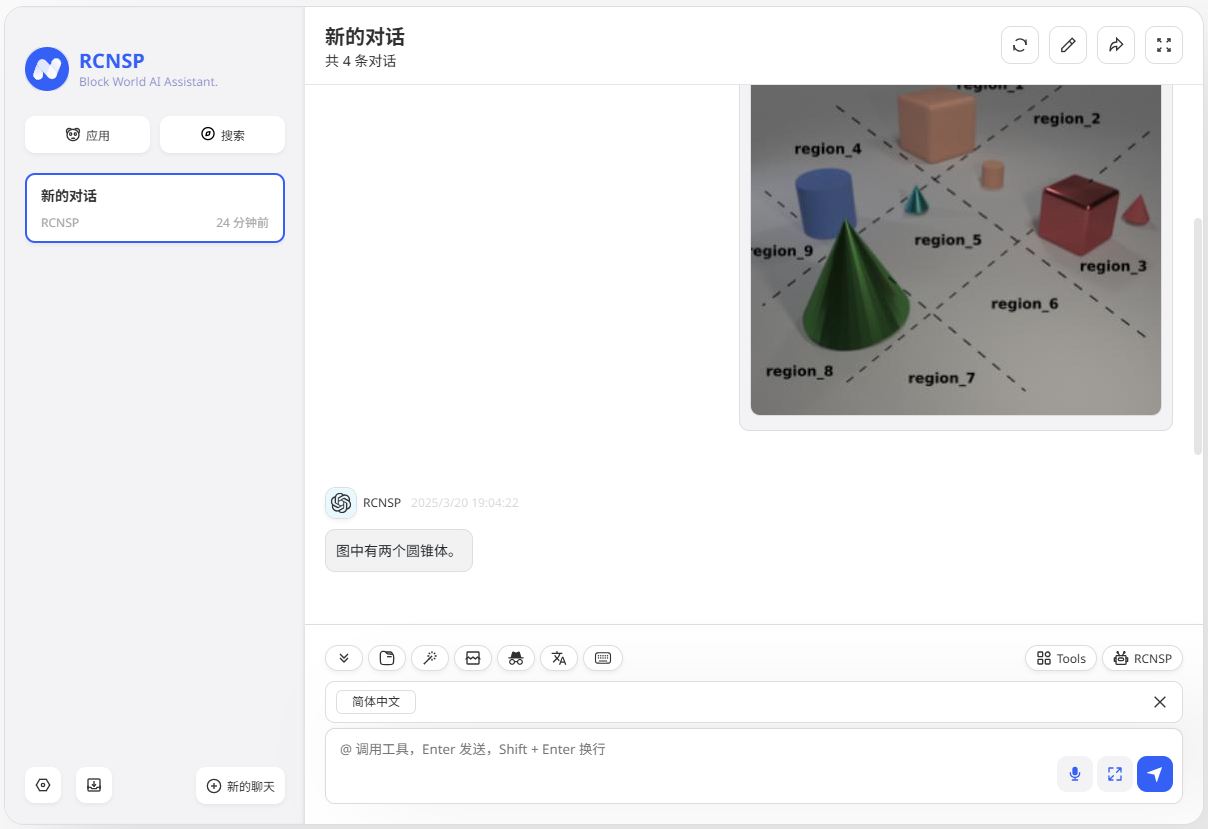
\includegraphics[scale=0.3]{figures/question.png}
    \caption{上传图片并提问后的效果}
    \label{fig:question}
\end{figure}
\begin{figure}[h]
    \centering
    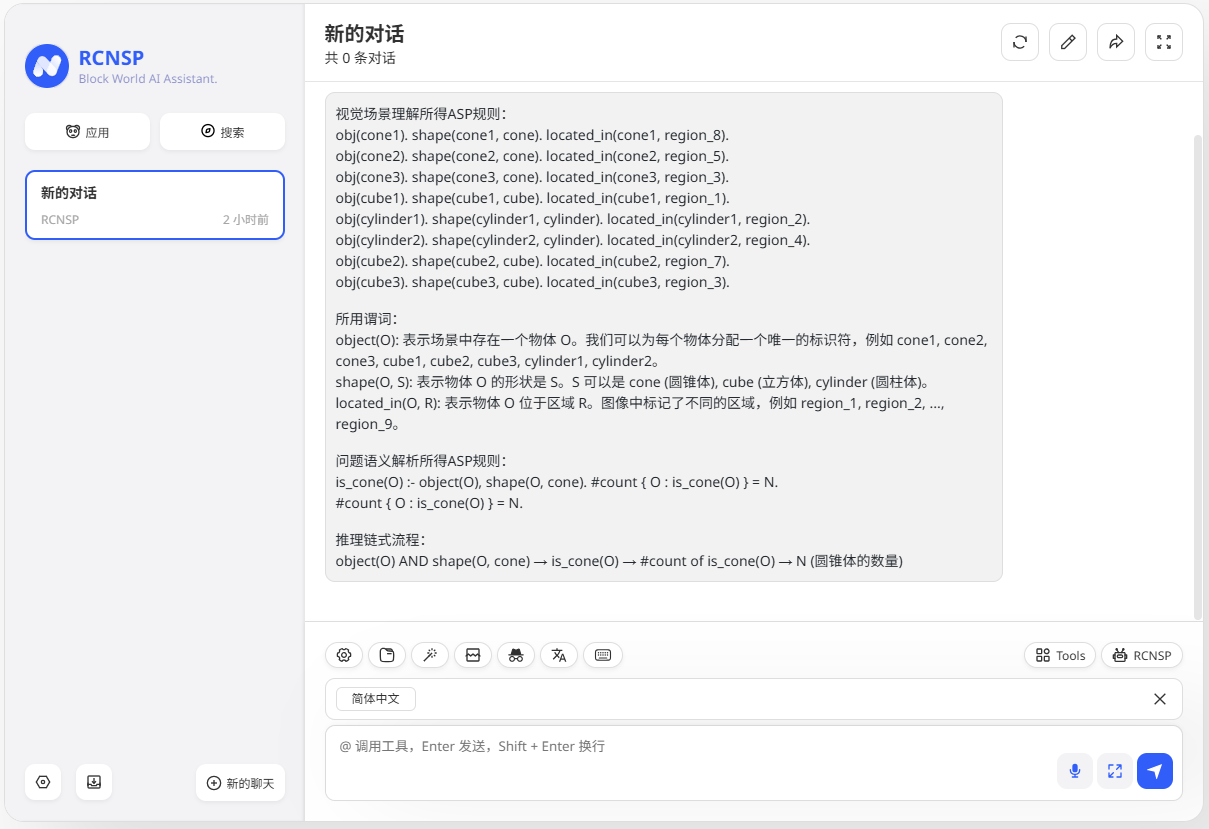
\includegraphics[scale=0.3]{figures/reasoning_path.png}
    \caption{逻辑链条展示}
    \label{fig:answer}
\end{figure}
\subsection{数据集自定义生成}
数据集自定义生成的前端控制台如图\ref{fig:dashboard}所示,用户可以在控制台中自定义一系列构建积木世界VQA数据集所需的参数。用户点击
“生成”按钮后,系统将会使用这些参数向后台的数据集构造工具POVQAD-Builder发起调用,进而构造数据集。
\begin{figure}[h]
\centering
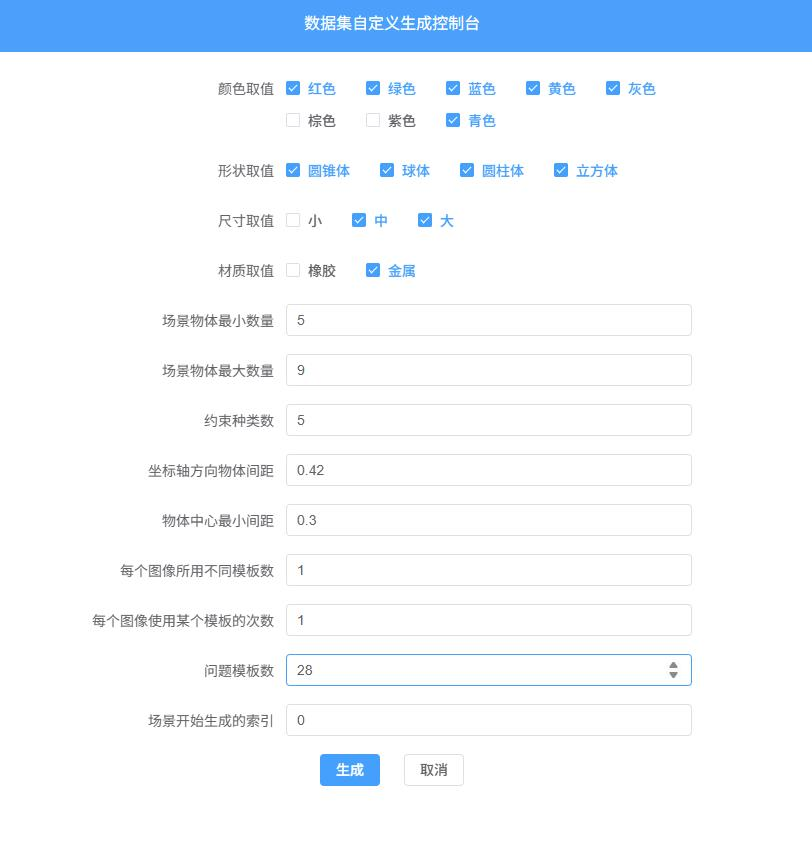
\includegraphics[scale=0.5]{figures/dashboard.jpg}
\caption{数据集自定义生成控制台}
\label{fig:dashboard}
\end{figure}
下面将从约束生成、图像及场景生成、问题生成和主控程序四个方面对POVQAD-Builder的实现细节进行介绍。
\subsubsection{约束生成}
系统约束模板存储在\texttt{ConstraintTemplates}文件夹中,所有的约束模板内容见附录\ref{appendix:constraints},
定义了场景中对象的数量、属性(如颜色、形状、材质)以及对象之间的关系。
例如,一个模板可能要求场景中必须包含两个红色球和一个蓝色立方体。此后,系统通过\texttt{generateEnvironment}
函数随机选择一个约束模板,并根据模板生成具体的约束。
生成的约束存储在\texttt{environment\_constraints}文件夹中,供后续场景生成阶段使用。

最终输出的约束文件以JSON格式存储,每个约束文件描述了场景中对象的数量、属性范围以及对象之间的关系,例如:
\begin{lstlisting}
{
  "num_objects": 5,
  "object_types": ["sphere", "cube"],
  "colors": ["red", "blue", "green"],
  "relationships": ["left", "right", "behind"]
}
\end{lstlisting}
\subsubsection{图像及场景生成}
图像及场景生成阶段的主要任务是根据约束生成场景,并使用Blender渲染工具生成场景图像和对应的场景描述文件(JSON格式),分为场景生成、场景关系计算和图像渲染三个环节。

场景生成中,程序根据约束文件随机生成场景中的对象及其属性(如形状、颜色、材质、大小、位置)。
使用\texttt{add\_objects}函数将对象添加到场景中,并确保对象之间不重叠。
使用\texttt{check\_visibility}函数检查对象是否在图像中可见,避免生成无效场景。

场景关系计算中,使用\texttt{compute\_all\_relationships}函数计算场景中对象之间的空间关系(如“左边”、“右边”、“前面”、“后面”)。
这些关系存储在场景描述文件中,供后续问题生成阶段使用。

图像渲染中,程序调用Blender的渲染功能生成场景图像。渲染参数(如分辨率、光照、摄像机角度)通过命令行参数控制。
渲染完成后,图像存储在指定的输出目录中。

最终输出Blender渲染的场景图像文件,命名形如\texttt{scene\_0001.png},以及场景描述文件。
场景描述文件以JSON格式存在,描述场景中每个对象的属性和对象之间的关系。以下是一个场景描述文件内容的示例:
\begin{lstlisting}
{
    "objects": [
      {"shape": "sphere", "color": "red", "material": "rubber", "position": [1.2, 0.5, 0.3]},
      {"shape": "cube", "color": "blue", "material": "metal", "position": [-0.8, 0.2, 0.1]}
    ],
    "relationships": {
      "left": [[0, 1]],
      "right": [[1, 0]]
    }
}
\end{lstlisting}
\subsubsection{问题生成}
问题生成阶段的任务是基于场景描述文件生成问题和答案。问题的生成基于预定义的模板,确保问题具有逻辑性和多样性。

实现细节上,问题模板存储在\texttt{CLEVR\_POC\_templates}文件夹中,定义了问题的结构和逻辑。模板支持多种问题类型,包括:
\begin{enumerate}[nosep]
\item 计数问题:如“场景中有多少个红色的球?”
\item 比较问题:如“哪个物体更大,红色球还是蓝色立方体?”
\item 查询问题:如“场景中左边的物体是什么形状?”
\end{enumerate}

问题生成时,程序通过\texttt{generate\_question}函数读取场景描述文件,并根据模板生成问题。
每个问题模板包含占位符(如\{color\}、\{shape\}),程序会根据场景信息替换占位符生成具体问题。

此后进行答案生成时,
程序根据场景描述文件计算问题的答案。
例如,对于问题“场景中有多少个红色的球?”,程序会遍历场景中的对象,统计符合条件的对象数量。

最终,输出JSON格式的问题文件,包含生成的问题(自然语言形式)、答案和问题的ASP程序,一个示例如下所示:
\begin{lstlisting}
{
  "question": "How many red spheres are there?",
  "answer": 2,
  "program": [
    {"function": "filter_color", "inputs": ["red"]},
    {"function": "filter_shape", "inputs": ["sphere"]},
    {"function": "count", "inputs": []}
  ]
}
\end{lstlisting}
\subsubsection{主控程序}
主控程序负责协调上述三个阶段的执行,并控制数据集的规模和划分。

主控程序通过命令行启动,系统将用户在控制台输入的参数以命令行参数的形式加以利用,发起对主控程序的调用,进而开始构造数据集。
示例命令如:
\begin{lstlisting}
python generate_dataset.py --num_train 10000 --num_val 2000 --num_test 2000 --resolution 320x240
\end{lstlisting}
主控程序依次调用约束生成、数据生成和问题生成模块。渲染完成后,程序会清理临时文件,确保生成过程高效。

最终,程序输出完整数据集,包括包括训练集、验证集和测试集,每个数据集包含以下内容:
场景图像(PNG格式)、场景描述文件(JSON格式)、问题文件(JSON格式,)。
\subsection{临机生成部分可见积木世界图像}
临机生成部分可见积木世界图像的控制台如图\ref{fig:blockworld-generation}所示。用户可以选择物体属性的可取值,并自定义
场景中物体的最小和最大个数,并可以自然语言形式输入用户认为其想要的部分可见积木世界中应满足的空间约束。
相关实现同前述数据集自定义生成大致相同,理论实现也已在本文第三章中予以介绍,此处不再赘述。
\begin{figure}[h]
\centering
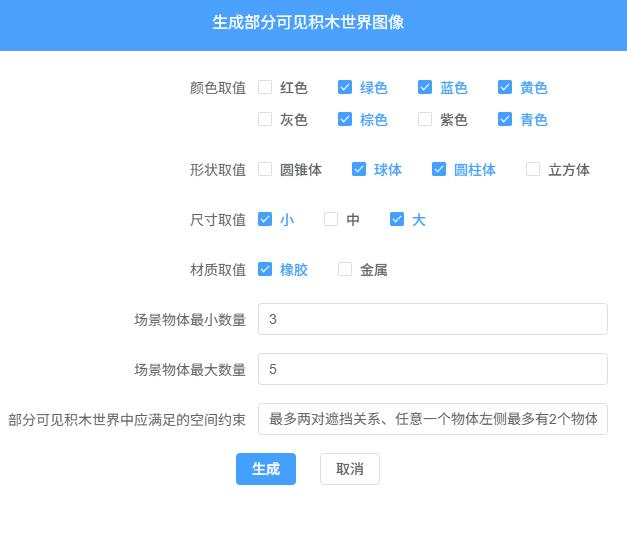
\includegraphics[scale=0.7]{figures/blockworld-generation.jpg}
\caption{生成部分可见积木世界图像控制台}
\label{fig:blockworld-generation}
\end{figure}
\section{集成测试}
系统的部署运行环境的硬件配置如下:CPU为Intel Core i9-12900K,内存为128GB,显卡为2张NVIDIA GeForce RTX 4090并联,操作系统为Ubuntu 20.04 LTS;
开发工具为IntelliJ IDEA、IntelliJ Pycharm和Microsoft Visual Studio Code。

前述需求中,需要通过测试以量化评估的主要为性能需求。因此,本文通过压力测试,对系统的性能进行量化评估。
本文使用JMeter工具进行压力测试。JMeter 是一种开源压力测试工具,可用于对Web应用程序、FTP服务器、数据库等进行性能测试。JMeter可以模拟多个用户同时访问服务器,以此来测试服务器的性能。
此外,使用SkyWalking对整个应用进行性能监控。图\ref{fig:SkyWalking}为SkyWalking对本系统中语义解析服务的监控面板,在其中可以直观监测服务的平均响应时间、成功率、每分钟调用数等信息。
\begin{figure}[h]
    \centering
    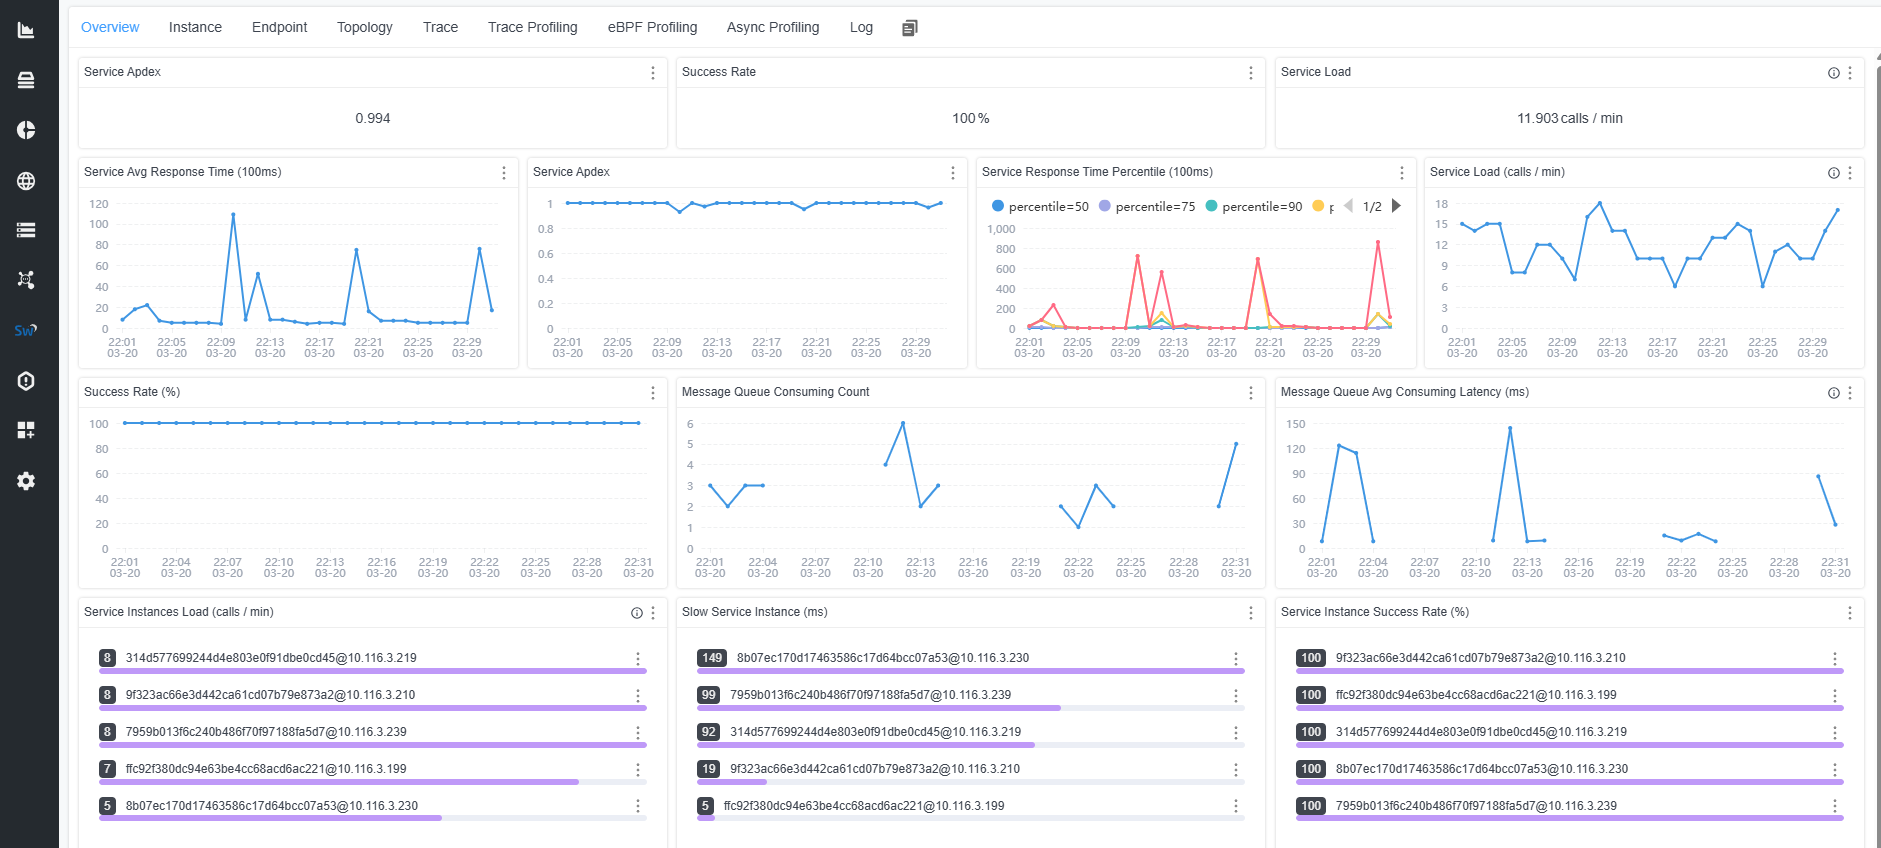
\includegraphics[width=\textwidth]{figures/SkyWalking.png}
    \caption{链路监控面板}
    \label{fig:SkyWalking}
\end{figure}

本文使用第三章中构造的数据集作为测试数据,测试的接口为用户交互接口。在开发各个接口时,已经在各个接口上设置了监控埋点。在SkyWalking中,能够看到各个接口的
调用次数,以及接口的响应时间等信息。即便是只对某一个接口发起模拟请求,进行压力测试,也可以通过SkyWalking来查看其它所有相关接口的相关参数。
用户交互接口处于整个调用链路的起点,对其进行压测,能够观测到整个VQA系统在执行一次任务时,所有相关接口的情况,故对其进行压测。

首先,确定压测目标。本系统作为一个原型系统,拟定的用户群体规模上限在50人左右,这一人数也是常见的课堂容量,则可以假设并发用户数目标为40人。通过对ChatGPT、DeepSeek、豆包等现有的
聊天机器人的使用的观察,发现目前普遍限制同一用户在同一时刻只能进行一个对话,若在原有对话仍在生成答案的同时,切换到新对话,将会导致原有对话的生成中断。
所以,本原型系统在压测目标上,设置每个用户的线程数都为1。
对以上各个接口,压测时长设置为30分钟。各用户线程加载,选用阶梯式加载的方式,随着时间推移,逐步增加并发用户数,以便观察系统在压力逐步增大时的性能变化。

其次,执行压测。在压测过程中,实时监控接口的性能指标,包括响应时间、吞吐量和错误率,同时监控系统的CPU使用率、内存使用率。

最终测试结果见表\ref{tab:test_result}。在38个并发用户下,系统响应整体较快,能满足大多数用户对视觉问答的需要。TPS表现整体稳定,错误率较低。总体而言,
压测结果表明,该系统能够满足其作为原型系统的要求,符合设计预期。
\begin{table}[h]
    \centering
    \renewcommand{\arraystretch}{1.3} % 调整行间距
    \begin{tabular}{|l|l|l|l|}
        \hline
        \textbf{参数} & \textbf{指标} & \textbf{参数} & \textbf{指标} \\
        \hline
        平均响应时间 & 8.3s & 90\%响应时间 & 6.9s \\
        \hline
        TPS & 38 & 错误率 & 0.5\% \\
        \hline
        CPU使用率 & 60.9\% & 内存使用率 & 56.8\% \\
        \hline
    \end{tabular}
    \caption{压力测试结果}
    \label{tab:test_result}
\end{table}
\section{本章小结}
本章围绕面向自动规划教学的积木世界VQA演示原型系统的设计与实现,
系统性地介绍了系统的需求分析、架构设计、数据库设计、安全策略、缓存机制、功能展示及性能测试等内容。

在需求分析部分,明确了系统既要满足教学演示的可用性与交互性,又需支持图像输入、语义解析、符号推理、可视化展示、自定义生成复杂度不同的演示数据集等关键能力,
并保障系统的安全性、扩展性与高可用性。系统架构方面,采用微服务设计理念,将语义解析、视觉理解、推理与生成等功能进行模块化分离,
各服务间通过API网关协同通信,提升系统灵活性与维护效率。

数据库设计涵盖用户、规则、对话与日志四类数据,为系统运行提供了坚实的数据支持。为兼顾性能与稳定性,
系统采用本地缓存与Redis分布式缓存结合的两级缓存架构,在提升响应速度的同时有效降低了后端负载。
此外,系统引入了包括SHA-256、AES、HTTPS、JWT等在内的多种安全技术手段,保障用户数据安全与系统抗攻击能力。

前端采用Vue框架构建,结合Element UI 与 Axios 实现组件化设计与前后端通信,并提供逻辑链条可视化、语音输入、多模型切换等便捷功能,
增强了系统的可交互性与教学可视性。在集成测试中,借助JMeter和SkyWalking对系统性能进行了定量评估,
测试结果表明本系统在多用户并发下仍保持较好稳定性和响应效率,能够满足预期的课堂演示环境下进行积木世界VQA时的用户并发量要求和响应延迟要求,
验证了其作为教学演示型原型系统的可用性与实用价值。

综上所述,本章实现了一个面向自动规划教学的积木世界VQA演示原型系统,为教师在自动规划课程教学过程中进行直观演示奠定坚实基础。